\chapter{Экспериментальный раздел}
\label{cha:research}
    В данном разделе будут проведены эксперименты для проведения 
    сравнительного анализа алгоритмов по затрачиваемому процессорному 
    времени и максимальной используемой памяти.
% и количеству максимально затрачиваемой памяти
    \section{Сравнительный анализ на основе замеров времени работы алгоритмов}
        В рамках данного проекта были проведёны следующие эксперименты:

        1) сравнение алгоритмов поиска расстояния Левенштейна и Дамерау-Левенштейна
        на строках длиной от 0 до 5 с шагом 1 (рисунок~\ref{fig:1});
        
        2) сравнение алгоритмов \footnote{Замеры времени для рекурсивного алгоритма поиска расстояния Левенштейна
        на строках длиной от 0 до 975 с шагом 75 не проводились, так как уже на
        строках длиной 10 алгоритм работает 70 034 ms, что в 35 000 раз больше, 
        времени работы алгоритмов с использованием матрицы. Это связано с экспоненциальной асимптотикой
        времени выполнения данного алгоритма (пропорционально количеству
        рекурсивных вызовов).} поиска расстояния Левенштейна и Дамерау-Левенштейна
        на строках длиной от 0 до 1000 с шагом 50 (рисунок~\ref{fig:2}).
        
        Эксперимент проводился на стационаном компьютере с процессором
        Intel(R) Core(TM) i5-7200U CPU 2.50 GHz
        под управлением Debian 10 с 8 Гб оперативной памяти.

        Ниже предствалены графики зависимости времени работы алгоритмов от длины входных строк
        (рисунки~\ref{fig:12} и~\ref{fig:22}).

        Обозначения:\newline
            a) levNR - алгоритм Левенштейна без рекурсии.\newline
            b) levRNC - алгоритм Левенштейна с рекурсией и без кэша.\newline
            c) levRWC - алгоритм Левенштейна с рекурсией и с кэшем.\newline
            d) levDamR - алгоритм Дамерау-Левенштейна с рекурсией.\newline

    \begin{figure}[h!]
        \centering
        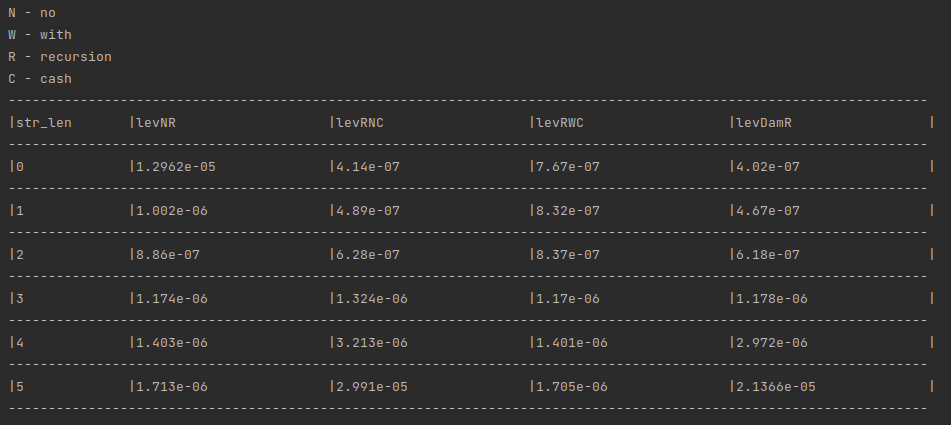
\includegraphics[scale=0.7]{img/TimeTable5Elems}
        \caption{Результаты замера времени на строках длиной от 0 до 5 в секундах}
        \label{fig:1}

        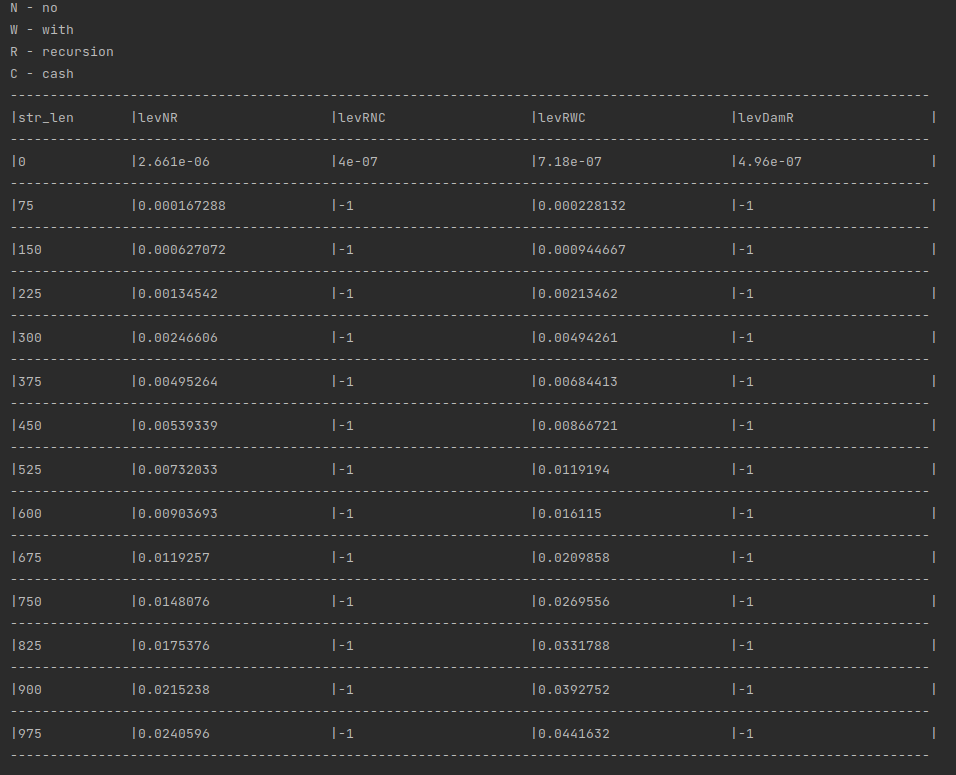
\includegraphics[scale=0.7]{img/TimeTable975Elems}
        \caption{Результаты замера времени на строках длиной от 0 до 975 в секундах}
        \label{fig:2}
    \end{figure}

    \begin{figure}[h!]
        \centering
        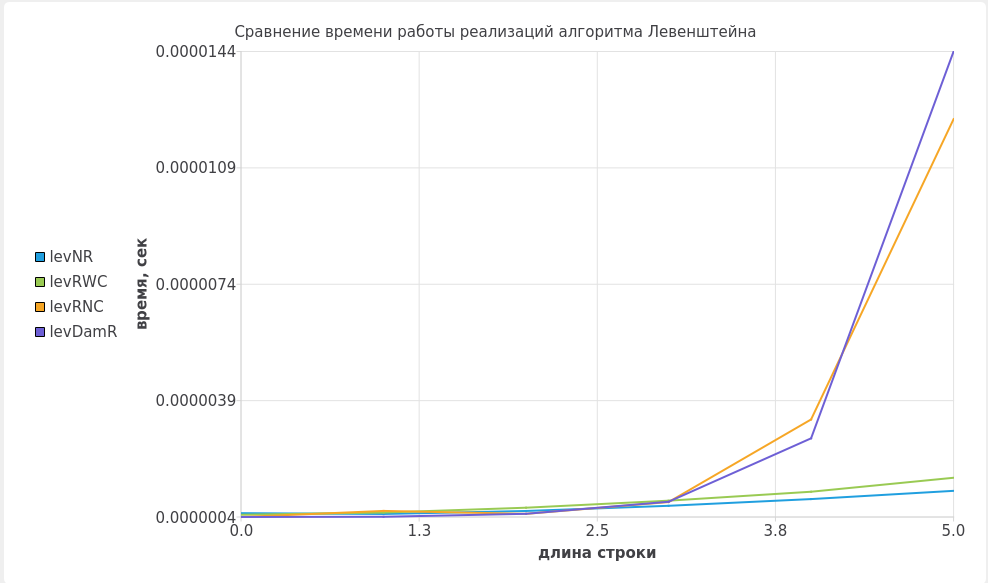
\includegraphics[scale=0.7]{img/smallGraphic}
        \caption{График зависимости времени работы алгоритмов от длин строк}
        \label{fig:12}

        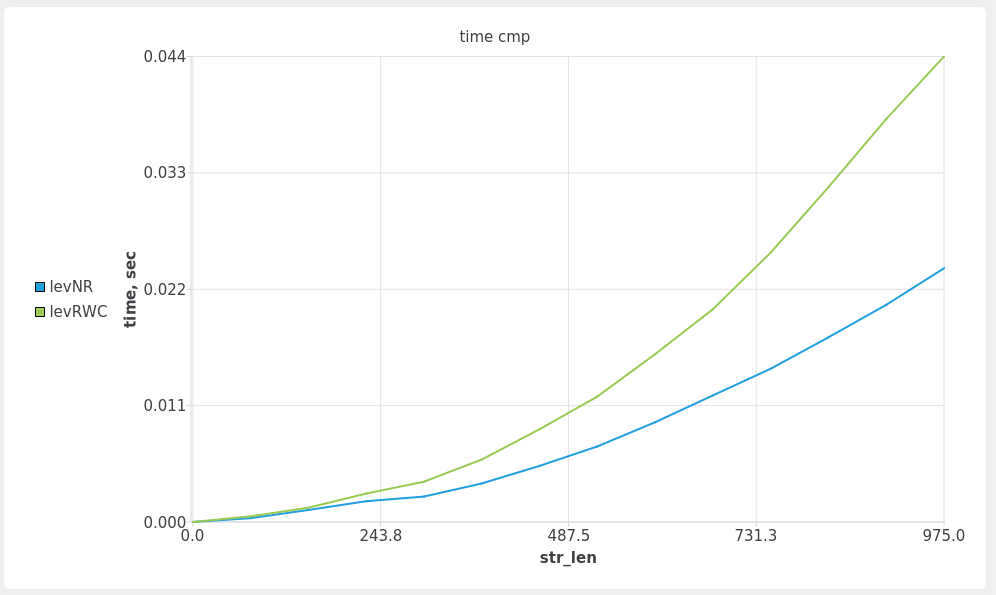
\includegraphics[scale=0.7]{img/LargeGraphic}
        \caption{График зависимости времени работы алгоритмов от длин строк}
        \label{fig:22}
    \end{figure}

    \section{Вывод}
        В данном разделе были поставлены эксперименты по замеру времени
        выполнения каждого из алгоритмов. По итогам замеров не рекурсивный 
        алгоритм нахождения расстояния Левенштейна оказался самым быстродействующим
        на длинах строк превышающих 3 на 136 \% быстрее, чем алгоритм поиска
        расстояния Левенштейна рекурсивно с заполнением матрицы и на 42 \%,
        чем реализация алгоритм поиска расстояния Дамерау-Левенштейна. На строках
        длиной менее 3х символов рекурсивная реализиция быстрее матричной, так
        как не выделяет в куче место под хранение матрицы.  
        
        По расходу памяти матричные алгоритмы проигрывают рекурсивному, так как
        максимальный размер используемой памяти имеет квадратичную ассимптотику
        (произведение длин строк), в то время как у рекурсивного - линейная (сумма длин строк).


\newpage